% This file was created by tikzplotlib v0.9.8.
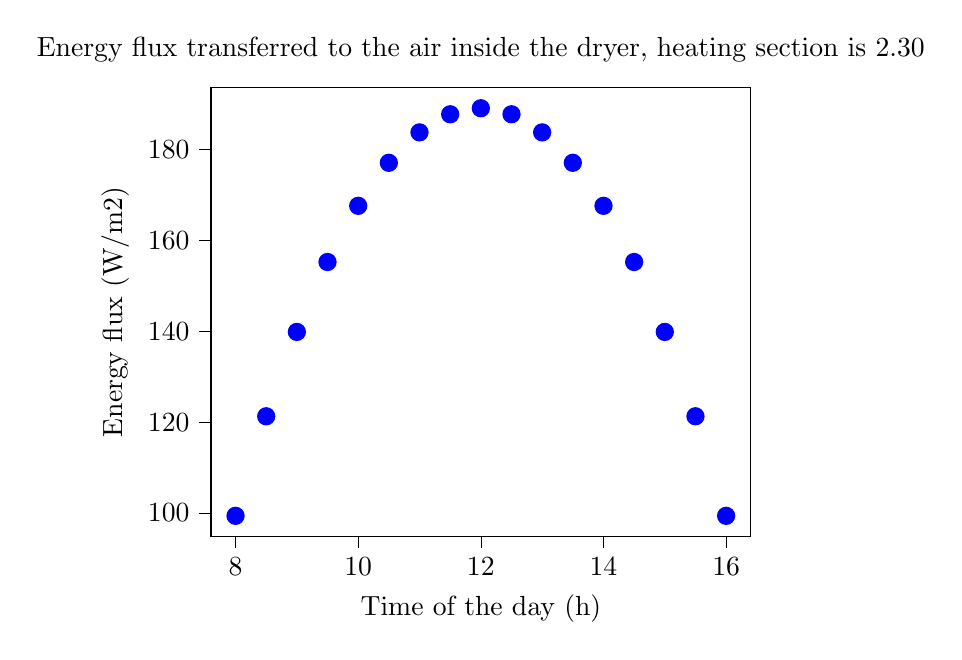
\begin{tikzpicture}

\begin{axis}[
tick align=outside,
tick pos=left,
title={Energy flux transferred to the air inside the dryer, heating section is 2.30},
x grid style={white!69.0196078431373!black},
xlabel={Time of the day (h)},
xmin=7.6, xmax=16.4,
xtick style={color=black},
y grid style={white!69.0196078431373!black},
ylabel={Energy flux (W/m2)},
ymin=94.908804442909, ymax=193.515146092901,
ytick style={color=black}
]
\addplot [semithick, blue, mark=*, mark size=3, mark options={solid}, only marks]
table {%
8 99.390910881545
8.5 121.283418686717
9 139.838638699674
9.5 155.21544134048
10 167.571089681677
10.5 177.040000980513
11 183.727943997678
11.5 187.710532227613
12 189.033039654265
12.5 187.710532227613
13 183.727943997678
13.5 177.040000980513
14 167.571089681677
14.5 155.21544134048
15 139.838638699674
15.5 121.283418686717
16 99.390910881545
};
\end{axis}

\end{tikzpicture}
